\documentclass{zc-ust-hw}

\usepackage{lipsum}

\name{SalahDin Ahmed Salh Rezk}
\id{202201079}
\course{Introduction to Electronics (CIE 212)}
\assignment{Lab Assignment 2}

\begin{document}

\maketitle

\begin{enumerate}
  \item \,
    \begin{figure}[h]
      \centering
      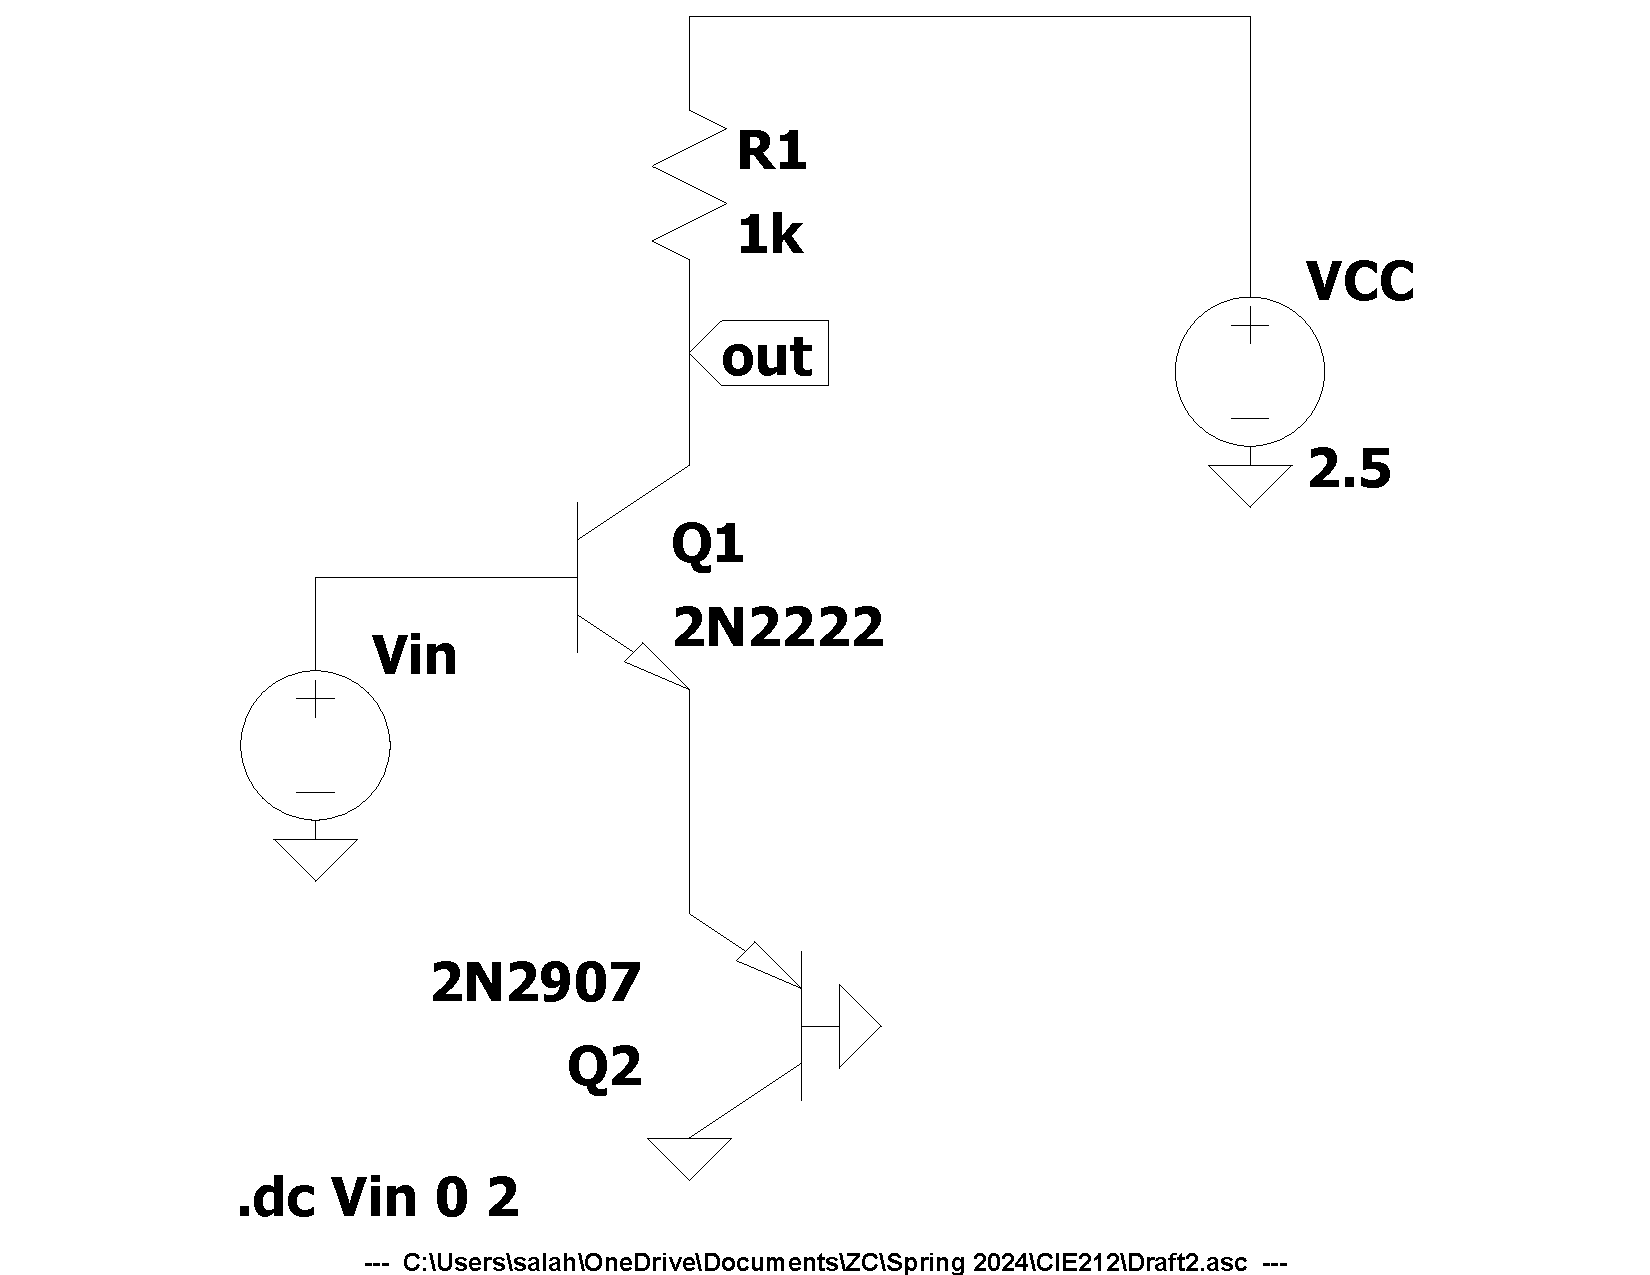
\includegraphics[width=0.5\textwidth]{figures/1-dc-circuit.pdf}
      \caption{}
    \end{figure}
    \begin{figure}[h]
      \centering
      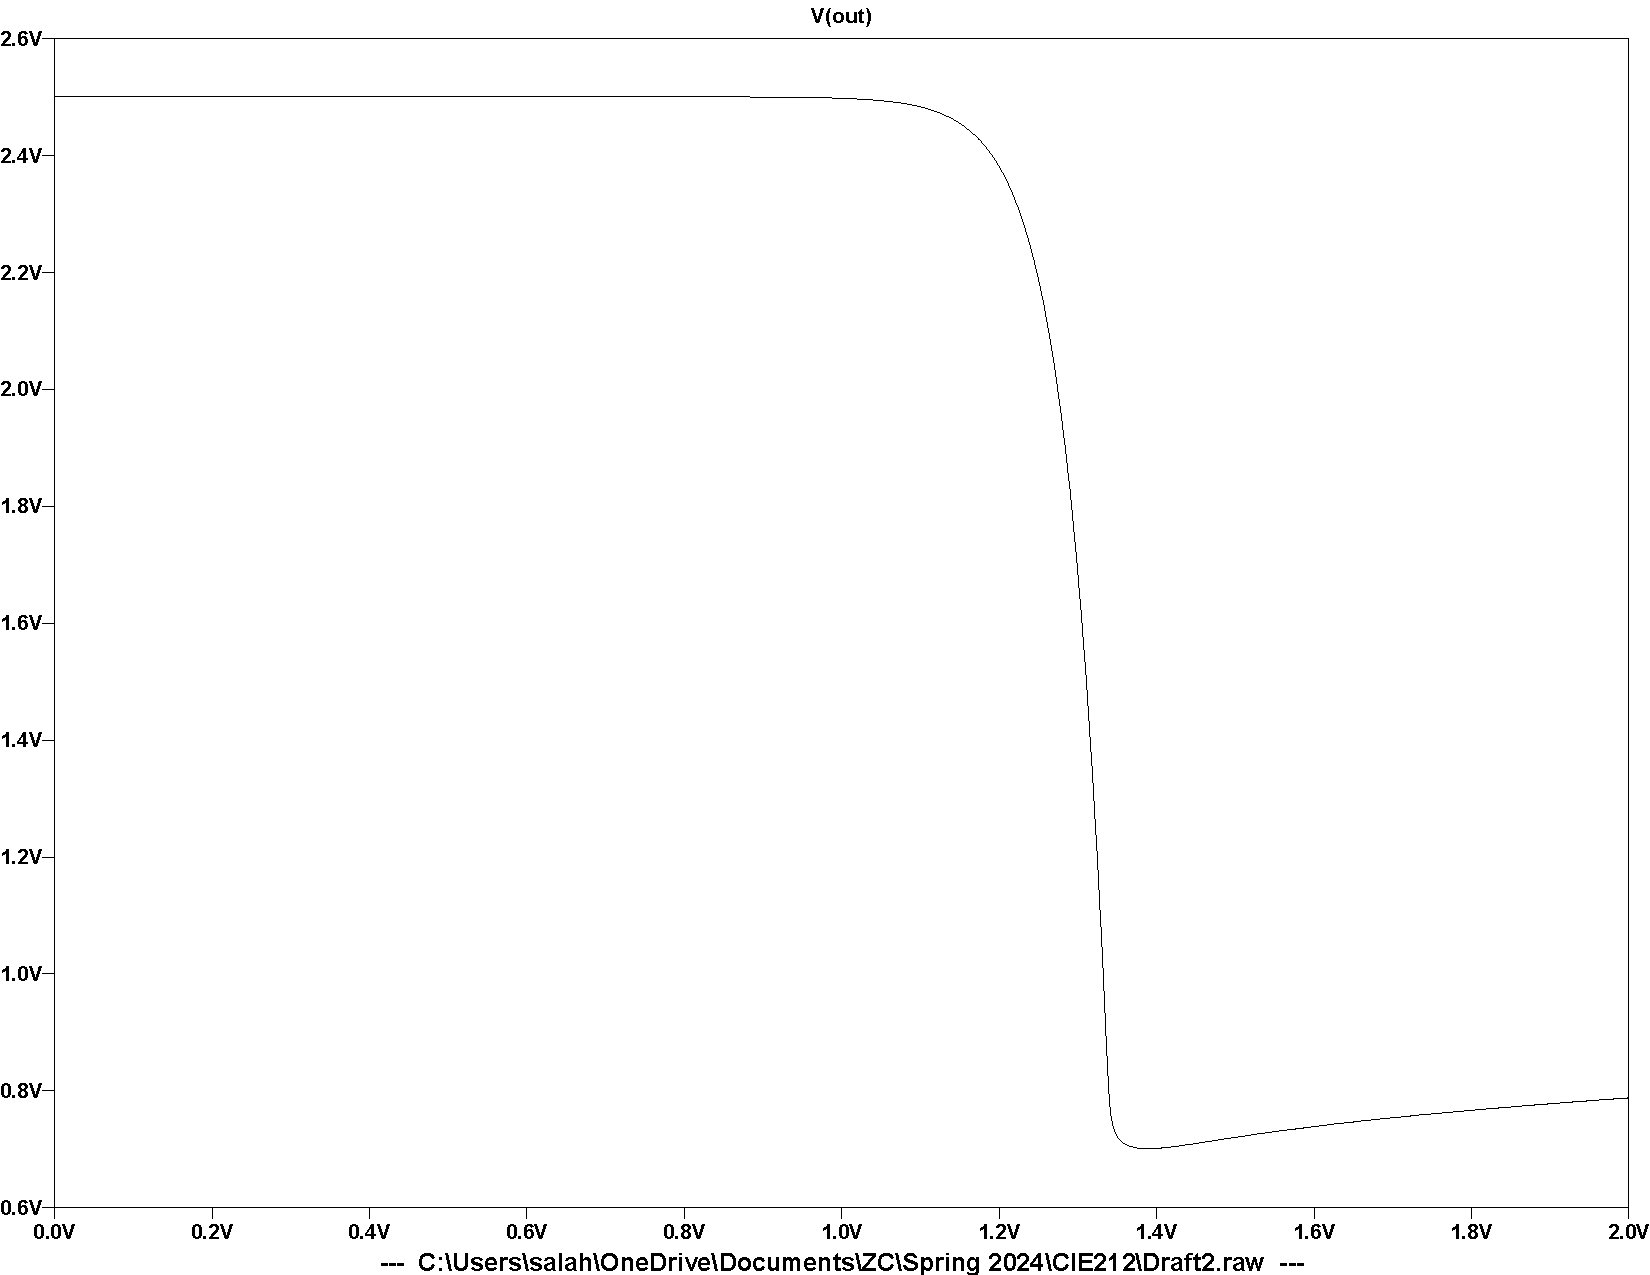
\includegraphics[width=0.5\textwidth]{figures/1-dc-graph.pdf}
      \caption{}
    \end{figure}

    The formula for transconductance is

    \[
      g=\frac{I_{c}}{V_{t}}
    .\]

    Calculating, we get a value of \( \frac{1}{50} \)S. Where the value of \(
    V_{t} \) is 1.5V, and the value of \( I_{c} \) is 0.5mA.

    \newpage

  \item \,
    \begin{figure}[h]
      \centering
      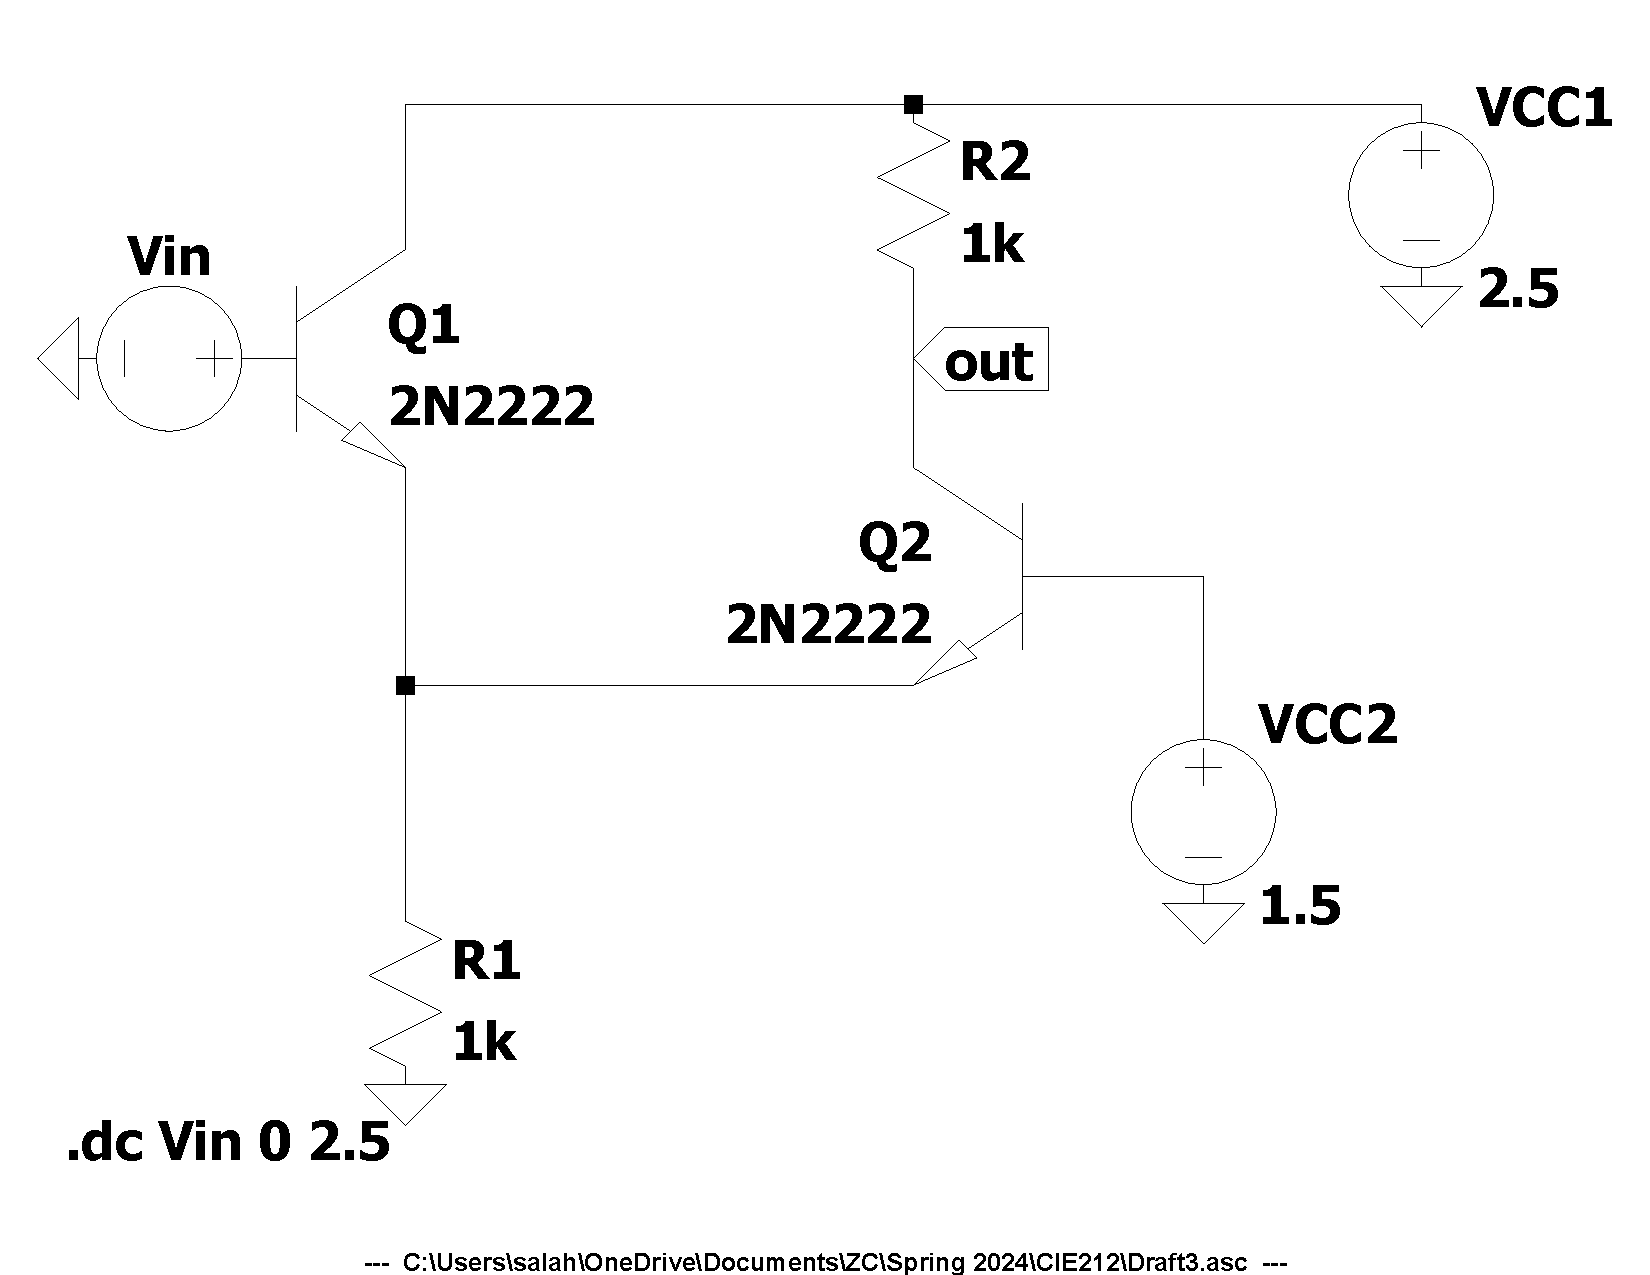
\includegraphics[width=0.6\textwidth]{figures/2-dc-circuit.pdf}
      \caption{}
    \end{figure}
    \begin{figure}[h]
      \centering
      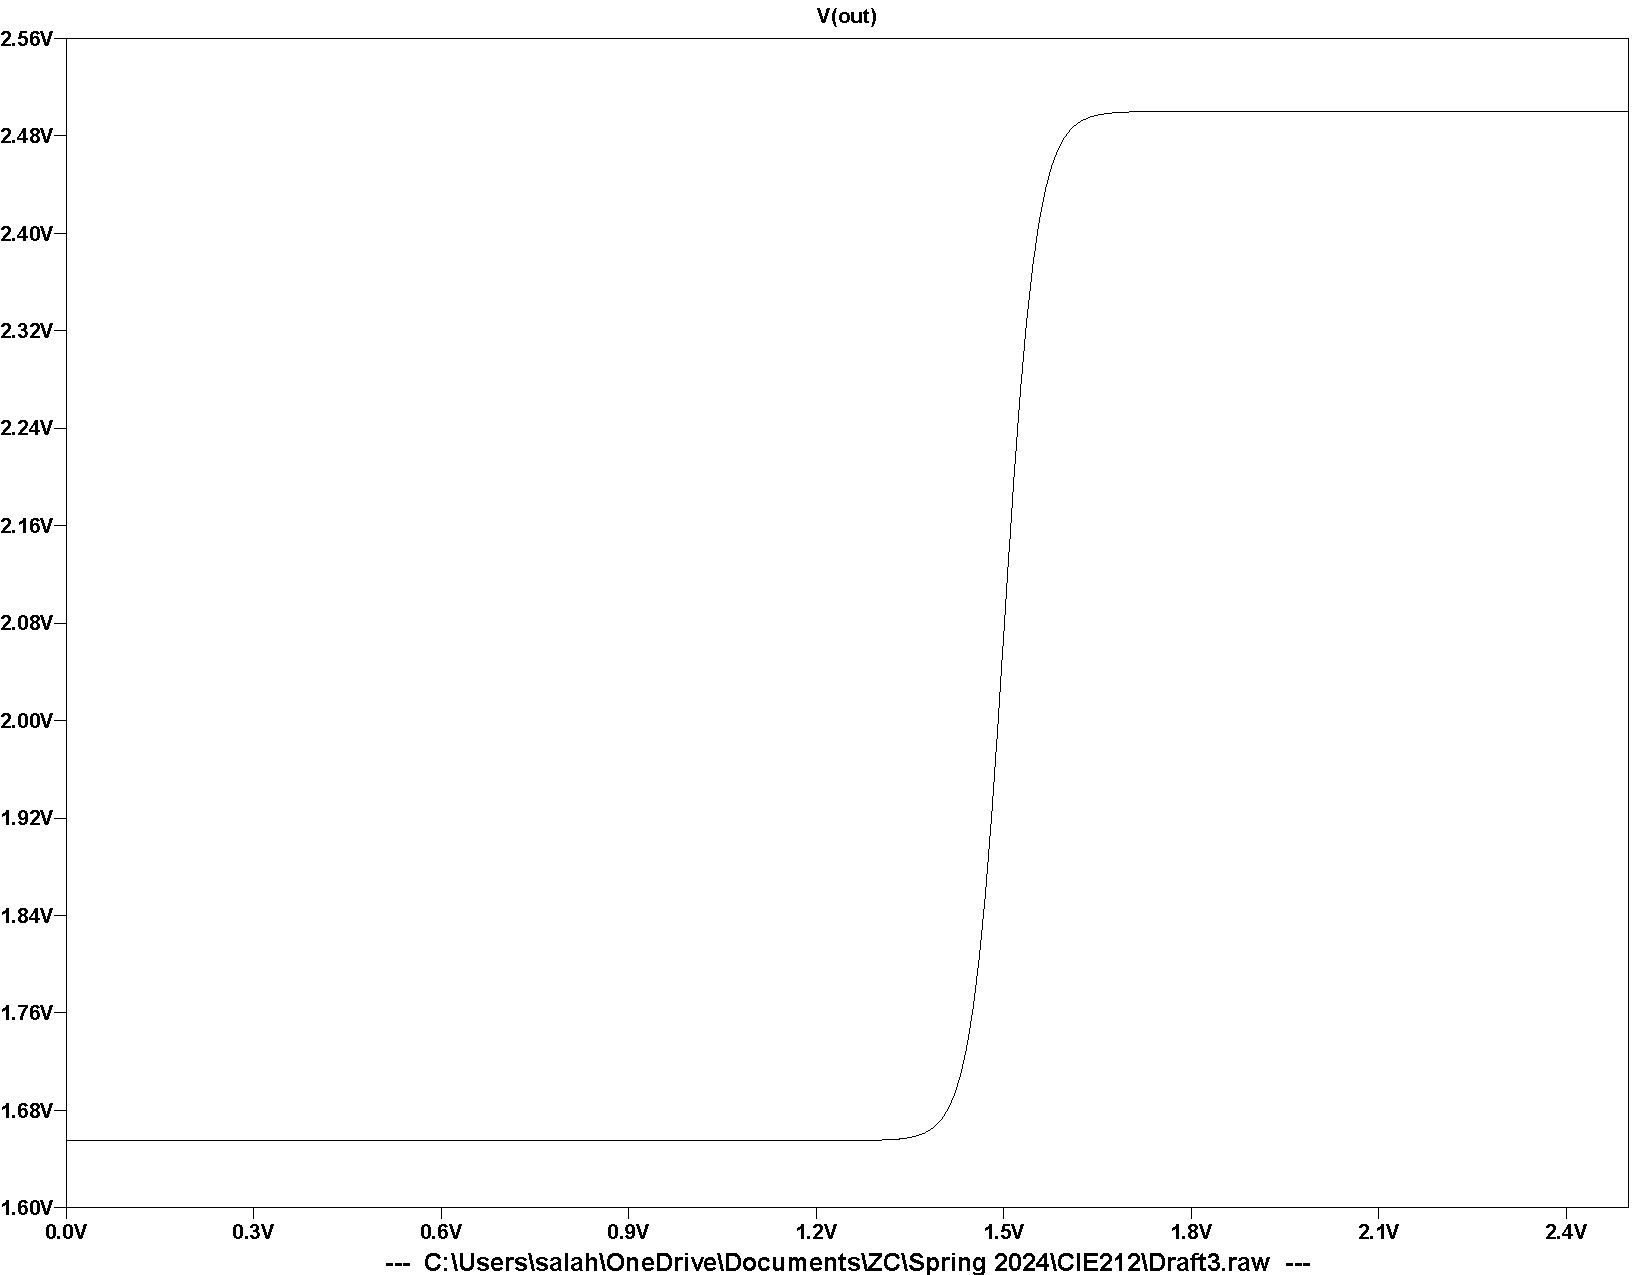
\includegraphics[width=0.6\textwidth]{figures/2-dc-graph.pdf}
      \caption{}
    \end{figure}

    The value of \( V_{t} \) is 1.5V, this can be intuitively explained by
    the fact that the circuit configuration is symmetric around \( Q_{1} \) and
    \( Q_{2} \) with \( Q_{2} \) base voltage of 1.5V.


\end{enumerate}

\end{document}
